\documentclass{vldb}

\usepackage{amsmath,amssymb}
\usepackage{stmaryrd}
\usepackage{graphicx}
\usepackage{color}

\newcommand{\comment}[1]{}
\newcommand{\compiler}{DBToaster}
\newcommand{\tinysection}[1]{\noindent{\bf #1.}}
\newcommand{\tuple}[1]{{\langle#1\rangle}}
\newcommand{\todo}[1]{\textcolor{red}{#1}}
\newcommand{\note}[1]{\textcolor{blue}{#1}}

\begin{document}
\title{Algorithmic Trading on Order Books with Embedded Queries and Synthesized
Stream Engines}
\numberofauthors{3}
\author{
\alignauthor
Oliver Kennedy\\
\affaddr{EPFL, Cornell}\\
\email{oliver.kennedy@epfl.ch}
\alignauthor
Yanif Ahmad\\
\affaddr{Johns Hopkins University}\\
\email{yanif@jhu.edu}
\alignauthor
Christoph Koch\\
\affaddr{EPFL}\\
\email{christoph.koch@epfl.ch}}
\maketitle

\begin{abstract}
Moo.
\end{abstract}

\section{Introduction}

\section{The DBToaster Platform}

The \compiler\ project investigates processing techniques and architectural
design for dynamic data management systems. Its two core research themes are
that of incremental query processing, and program synthesis where we can tailor
the design of system internals to yield lightweight, efficient data management
tools. Algorithmic trading, where specialized engines abound, is a natural use
case for \compiler. High-frequency data ingestion and the competitive advantage
of low latencies has led to widespread use of low-level code and
processing hardware such as FPGAs. We describe the computational and software
development aspects of the \compiler\ platform and toolchain below.

\tinysection{Dynamic Data Management}
\compiler\ constructs dynamic data management tools that process database
updates as incrementally as possible. Its query model is identical to that of
view maintenance \todo{[IVM citations]}, where given a query on a database, it
generates a program to maintain query results as the database changes. Its
novelty lies in the nature of this maintenance program, and its use of
\textit{agile} views and \textit{multi-level} view maintenance.
\todo{Blurb about agile views, etc.}

\tinysection{Query Engine Compilation and Synthesis} In its current incarnation,
\compiler\ acts as a one-shot compiler that transforms standard SQL queries into
incremental programs as described above. \compiler\ supports an extensible,
retargettable code generator that current has support for running incremental
programs in a variety of imperative or functional languages (C++, Java, OCaml),
as well as on massively parallel processing infrastructures (Hadoop, and
DBToaster Cumulus, a fine-grained shared-nothing streaming runtime currently
under development). In this demonstration, we will compile SQL queries to Java,
for use in our coarse-grained stream engine, Jasper (we describe this in
more detail below).

\todo{SQL queries, preaggregation, construction of incremental plan 
(polynomialization, delta transformation, simplification, repeat), low-level
compilation}

\todo{Diagram of platform: query, compiler, code generator backends, use of
generated code in runtimes}

\tinysection{Programming with DBToaster}

\todo{Embedded queries and query representation in languages (LINQ, Ferry, etc),
extraction and compilation, access query processing results, control flow and
notification}

\tinysection{The DBToaster Runtime}

\todo{Architecture diagram and components: data structures, compiling
operators, Jasper (a simple, generic stream processor), external windowing of
queries with Jasper+DBToaster}

\section{Algorithmic Trading}

\tinysection{Algorithmic trading workflow}

\todo{Architecture diagram}

\begin{figure}
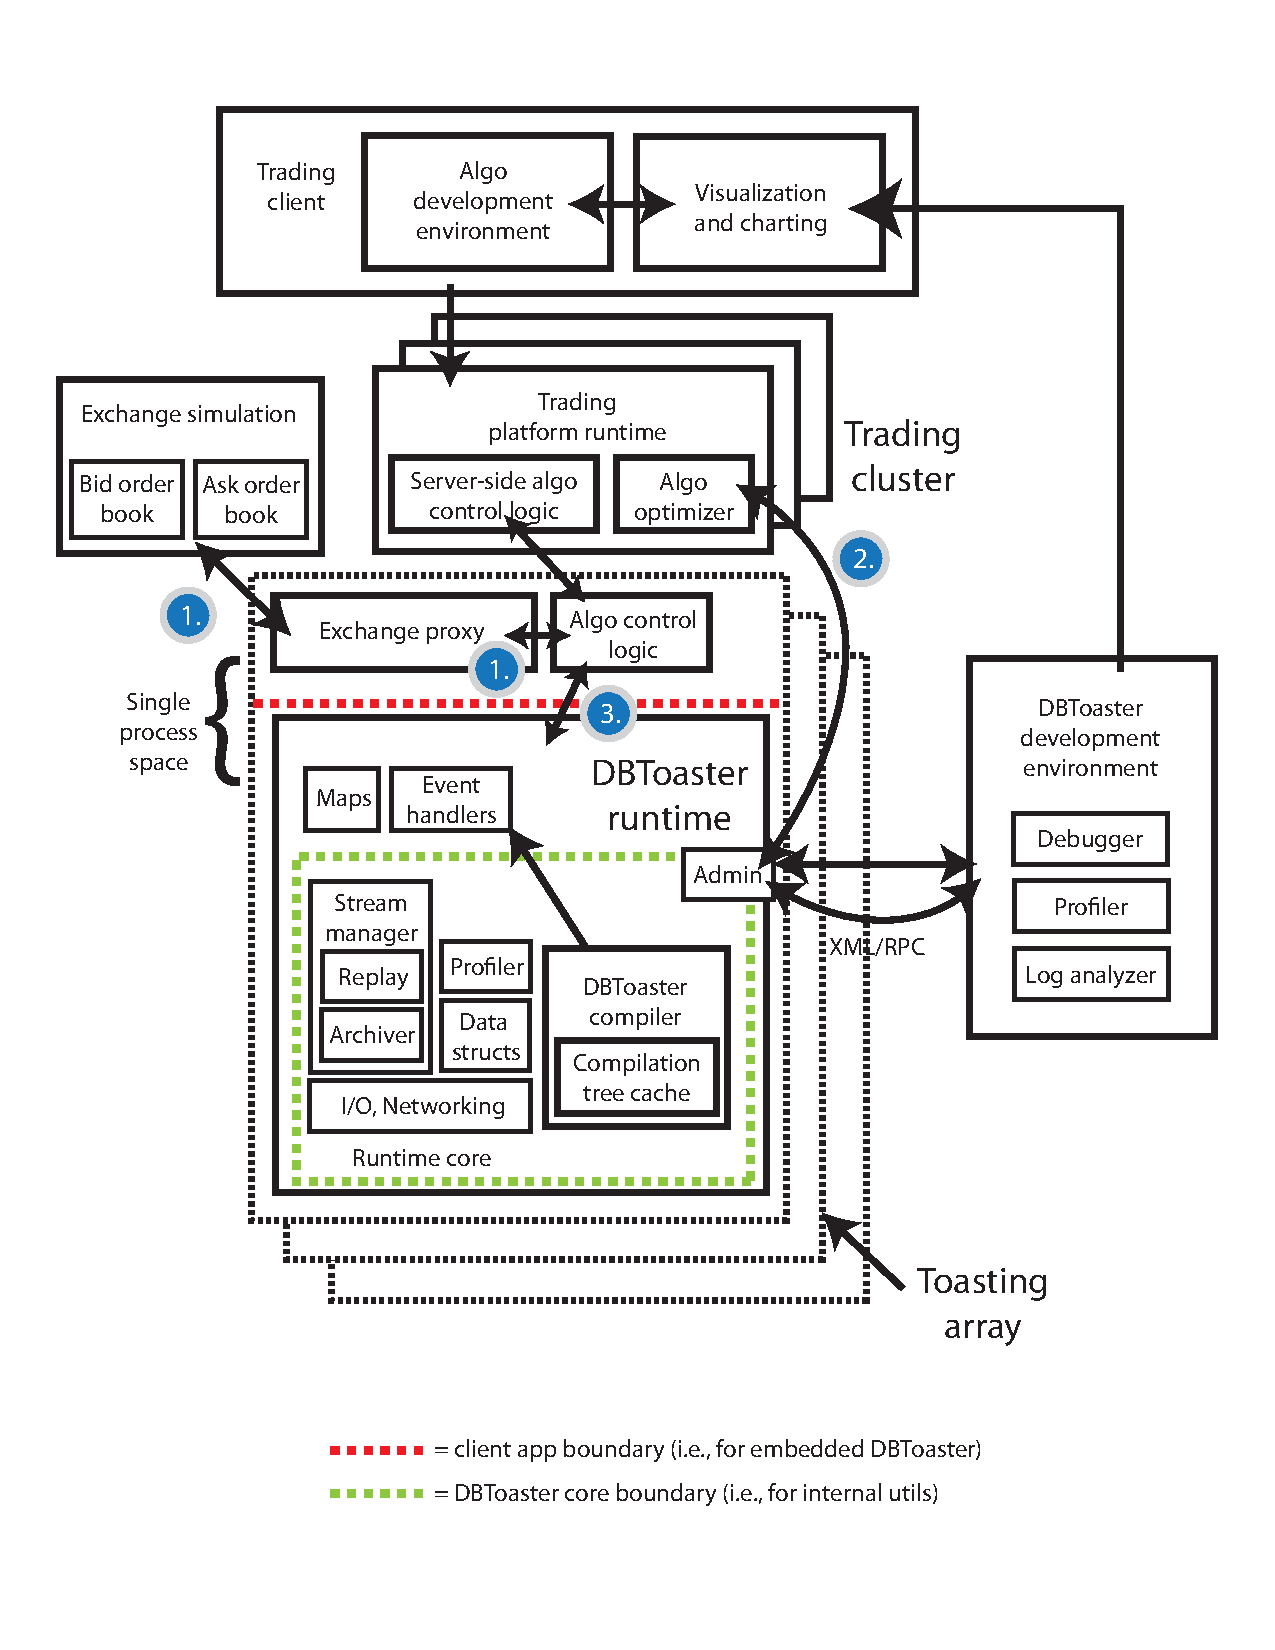
\includegraphics[scale=0.38]{figures/finapp}
\end{figure}

\tinysection{Electronic exchange}

\tinysection{Trading algorithms}

\tinysection{Trading workstation}

\begin{itemize}
  \item Example algorithms: VWAP, Ax finder, market making, icebergs, sniping.
  \item Advanced algorithms: combining level I and level II algorithms,
  combining alternate data sources, e.g. news feeds, twitter feeds. Would be
  nice to have learning algorithms and maintenance for them.
  \item Portfolio management.
  \item Exchange simulation: using histories to create alternate realities
  \item Algorithm simulation and backtesting: creating multiple agents that
  interact with each other
  \item Trading workstation: \todo{declarative visualization would be awesome..}
\end{itemize}

\section{Demo Scenario}

\todo{Demo screenshots}

\tinysection{Audience Participation}

\end{document}
